% Section 7.6 -- E6: noise (P2)
% Numbers from results/E6/E6_noise.csv (means over 10 instances per n).

\subsection{E6: Robustness to noise}
\label{sec:e6}

E6 asks what happens when angles found on a perfect simulator are run on a noisy device.
We take the noiselessly optimised angles for ten instances at $n = 6$ and $8$ and depths $p = 1, \dots, 4$, and evaluate them without re-optimising under depolarising noise: each two-qubit (CX) gate fails with probability $p_{\text{err}} \in \{0, 0.001, 0.005, 0.01\}$, and each single-qubit gate with probability $p_{\text{err}}/10$.
We use CUDA-Q's density-matrix simulator, which is exact, so the results contain no shot noise; at $p_{\text{err}} = 0$ every run reproduces the noiseless energy.

\begin{figure}[t]
  \centering
  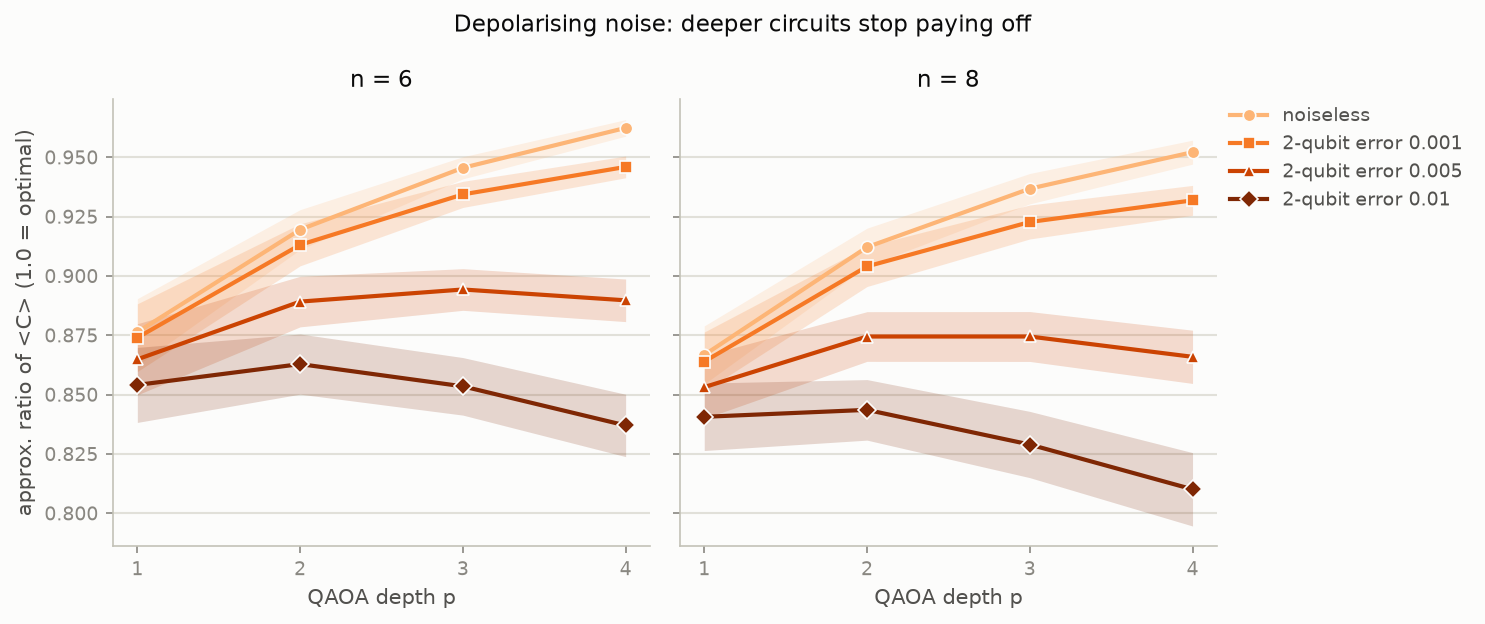
\includegraphics[width=\linewidth]{E6_noise.png}
  \caption{E6. Approximation ratio of the mean cost against depth for each two-qubit error rate, at $n = 6$ (left) and $n = 8$ (right). Bands show $\pm 1$ standard error.}
  \label{fig:e6}
\end{figure}

A small error rate costs little (Fig.~\ref{fig:e6}).
At $p_{\text{err}} = 0.001$ quality still improves with every layer and ends only $0.02$ below the noiseless value at $p = 4$ ($0.932$ against $0.952$ at $n = 8$).
At $0.005$ the improvement stops after two or three layers, at about $0.89$ for $n = 6$ and $0.874$ for $n = 8$.
At $0.01$ depth becomes harmful: at $n = 8$ the ratio falls from $0.841$ at $p = 1$ to $0.810$ at $p = 4$, and all ten instances end lower at $p = 4$ than at $p = 1$.
The success probability suffers more than the mean: at $n = 8$ and $p = 4$, $P(\text{opt})$ drops from $0.17$ without noise to $0.05$ at $p_{\text{err}} = 0.01$.

The cause is a trade-off between depth and gate count.
Each layer improves the ideal state, but also adds one $ZZ$ interaction, and so two CX gates, for every pair of jobs: 56 per layer at $n = 8$, and 224 at $p = 4$.
At $p_{\text{err}} = 0.01$, only $0.99^{224} \approx 10\,\%$ of runs pass through all of them without a two-qubit error.
Once the errors added by a layer outweigh its improvement, deeper circuits do worse, so the best depth depends on the hardware's error rate.
This noise model is simplified; Section~\ref{sec:discussion} discusses what it leaves out.
